\section{计算机视觉基础模型}
\label{sec:2_cv}

深度学习技术不仅推动着自然语言处理技术的发展与革命,其在早期更是在计算机视觉领域推动者各项技术从研究起步迈向成熟落地。相比于自然语言处理技术在近年来才迎来应用热潮,计算机视觉中的相关研究则早已应用到生产生活中。这也是目前大部分融合视觉信息的自然语言处理任务均应用预训练好的计算机视觉基础模型对图像进行编码的原因。

融合图片信息的神经机器翻译任务需要将图片信息输入到神经机器翻译模型中,因此同样需要采用神经网络方法对图片信息编码。针对不同的翻译模型选择合适的图片编码方法,能够提升视觉信息在翻译模型中的作用,从而帮助提升翻译模型的性能。目前ImgNMT中融合图片信息的方式主要可以分为三类:图片全局信息、图片动态局部信息以及视觉目标信息。本节,我们将主要针对这三类图片信息作用方式介绍其背后的计算机视觉基础模型。

% 基础模型在ImgNMT中的利用:
%   CNN:全局特征、栅格特征
%   R-CNN:视觉目标特征
%   visual grounding:(短语,视觉目标特征)

\subsection{卷积神经网络}
\label{sec:2_cnn}

卷积神经网络是目前计算机视觉领域最重要且最流行的方法之一,可以在计算机视觉的多个研究任务中发挥重要作用,例如图像分类、目标检测、人脸识别、语义分割等。早在20世纪90年代,杨·乐坤(Yann LeCun)等人发表论文提出了LeNet-5,成为奠定了现代卷积神经网络方法的基础框架\pcite{fukushima1980neocognitron,lecun1989handwritten,lecun1998gradient}。
现有的卷积神经网络,如AlexNet\pcite{krizhevsky2012imagenet},VGGNet\pcite{simonyan2015very},GoogLeNet\pcite{szegedy2014going},ResNet\pcite{he2016deep},DenseNet\pcite{huang2017densely}等模型,均是在LeNet-5的基础上通过加深网络层数、增加或改变非线性激活层、增加批数据归一化、增加通道数量等手段提升网络的泛化性能和对图像的表征能力。卷积神经网络不仅在计算机视觉领域得到广泛应用,在语音识别和自然语言处理的某些特定任务上同样得到了关注。在融合图像信息的多模态任务上,卷积神经网络更是用于表征图片信息或视频信息的必然选择。本节将以LeNet-5为例,详细介绍卷积神经网络的基本结构,以及应用到跨模态信息融合时的使用方式。

\begin{figure}[!htbp]
    \centering
    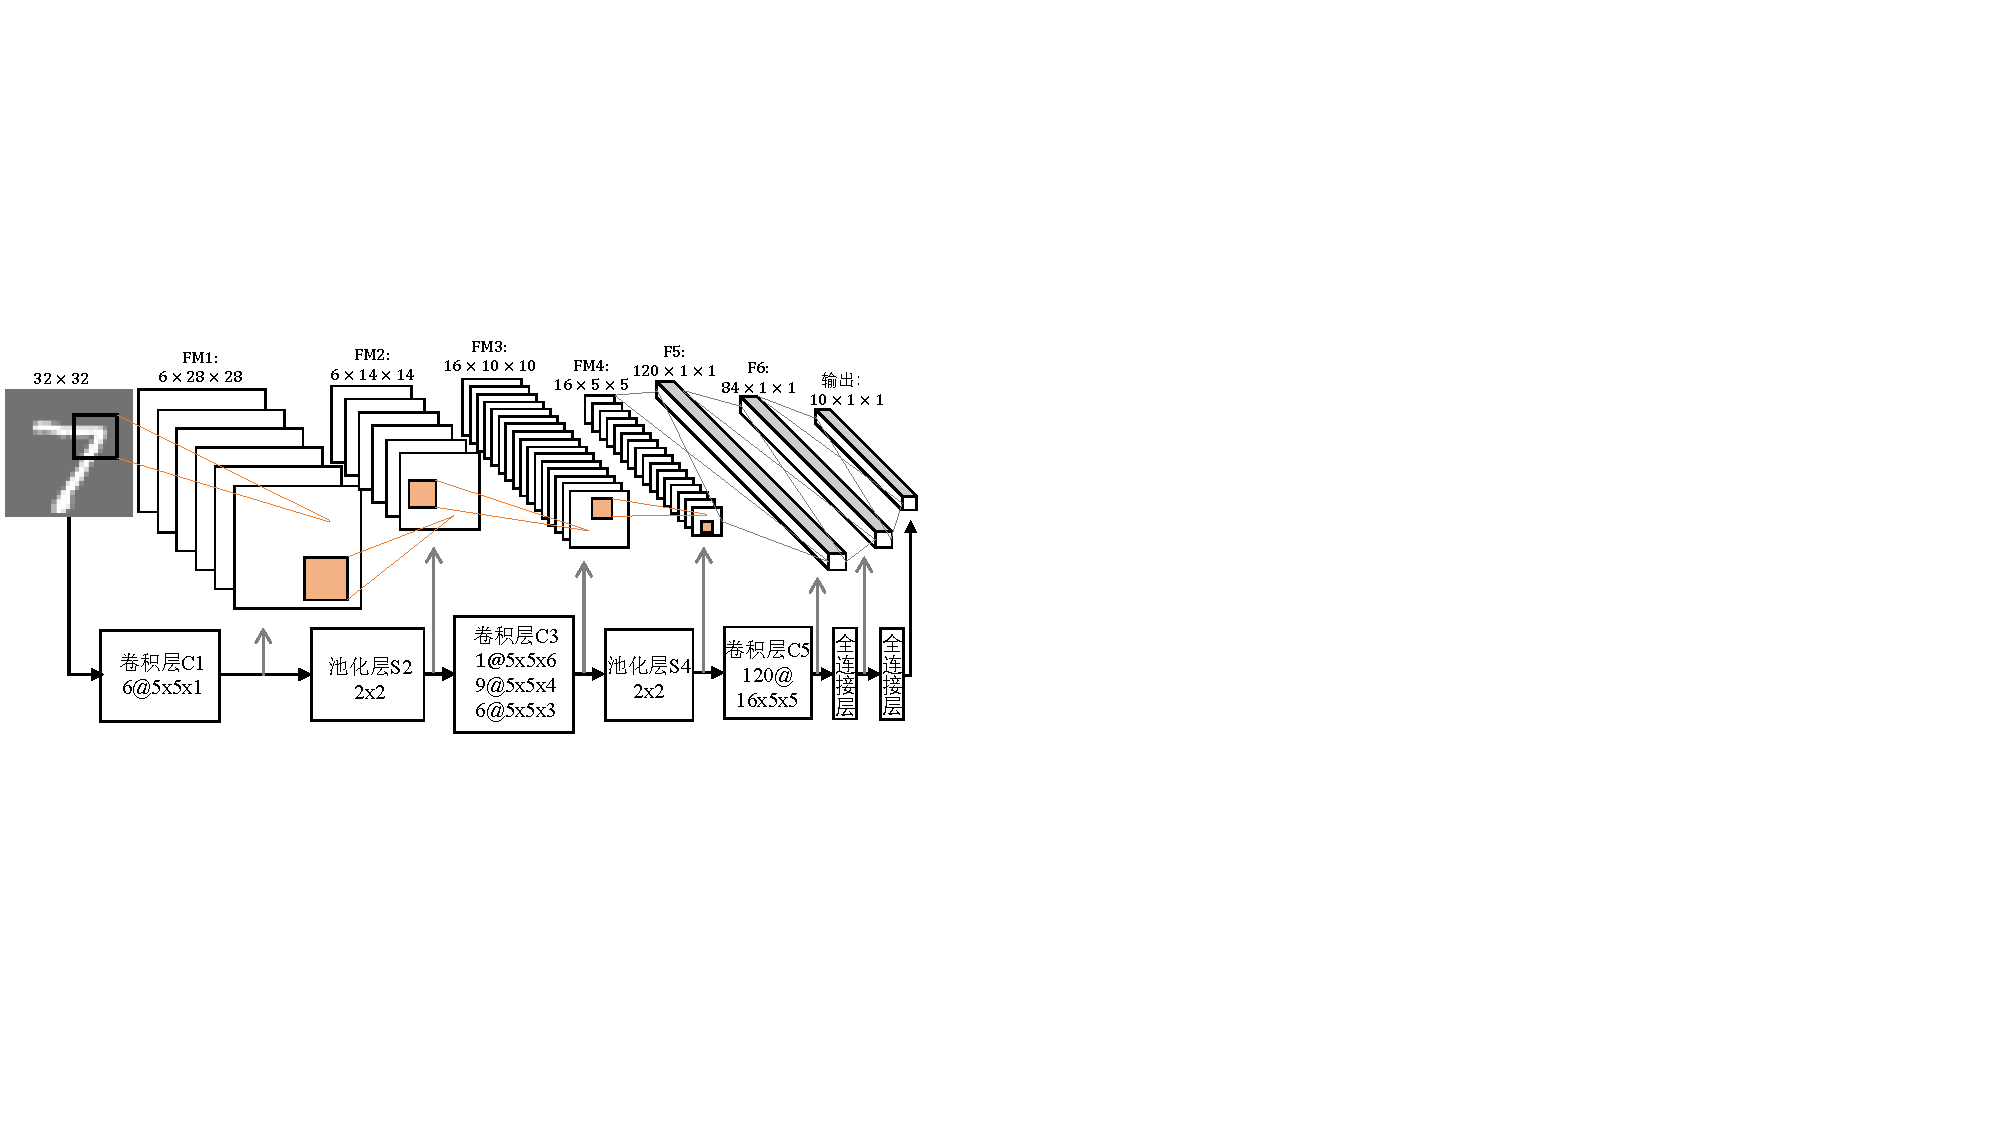
\includegraphics[scale=0.9]{Img/fig_2_lenet5.pdf}
    \bicaption{LeNet-5模型示意图}{Schematic diagram of the LeNet-5 model}
    \label{fig:2_lenet5}
\end{figure}
LeNet-5是最早的卷积神经网络模型之一,设计之初被用于手写数字识别任务。图\ref{fig:2_lenet5}展示了LeNet-5从输入图片到输出预测结果的模型工作简化图。LeNet-5共包含5层,包括两个卷积层(convolutional layer)C1、C3、C5,以及两个池化层(pooling layer)S2和S4。

{\sffamily 卷积层:}卷积层是CNN模型的核心模块,包含了整个模型的大部分参数。它可以对输入图像的局部区域进行加权求和从而得到图片的特征(feature)或特征图(feature map,FM),例如示例中经过卷积层得到的特征或特征图有FM1、FM3和F5。卷积层中卷积核(convolution kernel)大小和形状的选择能够影响卷积的效果。例如,图\ref{fig:2_lenet5}中卷积层C1中有6个$5 \times 5 \times 1$的卷积核,每个卷积核将图片中每个$5 \times 5$大小区域内的像素点加权求和得到输出特征图中的一个像素点,那么一个$32 \times 32$大小的图片经过卷积层C1后得到的特征图FM1的大小为$6 \times 28 \times 28$。经过卷积层后,图片的通道数可能会增加,图片的尺寸也可能变小。卷积层的设计可以很简单也可以非常的复杂,例如卷积层C3中包含了16个卷积核,其中各卷积核的尺寸为$5 \times 5$,但选取的特征图数量(图中包含6,4,3三种数量的差别)却各不相同。这说明卷积层的设计可以是非常灵活的,也因此对模型设计与研究人员的考验也是巨大的。

{\sffamily 池化层:}池化层一般也成为下采样层(subsampling layer),相当于一个过滤器,对图片或特征图执行降维操作,滤掉无用的像素点,帮助模型提取更高层次的特征。其原理是在输入特征图中一个局部区域内,按照选取最大值或计算平均值的方式为输出特征图增加一个新的像素点,也称最大池化(max pooling)和平均池化(average pooling)。例如图\ref{fig:2_lenet5}中的池化层S2的大小为$2 \times 2$,它在图片中对应区域内选取最大值或计算平均值后输出到特征图FM2中。区别于卷积层,池化层对输入特征图进行过滤像素时,一般不设置重叠区域,例如图中的池化层的尺寸和步长均为2,因此特征图经过池化层后特征图的尺寸变为原来的二分之一。

{\sffamily 全连接层:}全连接层(full connection layer)层中的每个神经元都连接着上一层的所有神经元。区别于卷积层和池化层将图片映射到隐层的特征空间中,而全连接层将隐层表示映射为图片的分布式特征表示,或经过非线性激活函数(一般采用softmax函数)得到样本的概率模型并预测样本的分类结果。例如图\ref{fig:2_lenet5}中最后的全连接层将图片特征F6映射为一个维度为10的向量中,每个维度的取值为0到1,代表着预测为0到9每个值的概率。

虽然LeNet-5的结构简单,但依旧展现了卷积神经网络能够学习并表征图片信息的能力。层数更深,网络结构更复杂,以及采用了更多新技术的新一代卷积神经网络能够表征更复杂的图像信息。在融合视觉信息的自然语言处理任务中,因文本输入与图片输入很难在一个模型中同时支持,因此通常采用特征融合的方式支持多模态输入。从一般的卷积神经网络的模型结构可以看到,选取图片特征的选择可以有很多种。例如图\ref{fig:2_lenet5}中FM4的尺寸为$16 \times 5 \times 5$,其中,在$5 \times 5$的特征图内仍保留着与源图片中的区域对应关系。因此FM4可看作是由$5 \times 5$个维度为16的特征组合而成,每个16维的特征表征了图片中对应的区域。这种保留了图片内局部空间信息的特征图一般称为栅格特征(grid feature)或局部特征(local feature)。在融合图片信息的神经机器翻译方法中,栅格特征一般可以作为图片输入序列输入到翻译模型中,通过注意力机制能够动态地关注到栅格特征中保留的局部空间信息。利用平均池化将栅格特征所代表的多个视觉特征融合为一个视觉特征,称作全局特征(global feature)。全局特征表征了图片的全局信息,通常可以用于初始化循环神经网络,或作为词向量等方式输入到神经机器翻译模型中。

% 要强调栅格信息保留了位置信息
% 这里最好直接举ResNet的例子,可以直接将残差连接的引入到现有机器翻译模型中

\subsection{目标检测方法}
\label{sec:2_object_detection}

\begin{figure}[!htbp]
    \centering
    \begin{subfigure}{\textwidth}
      \centering{
      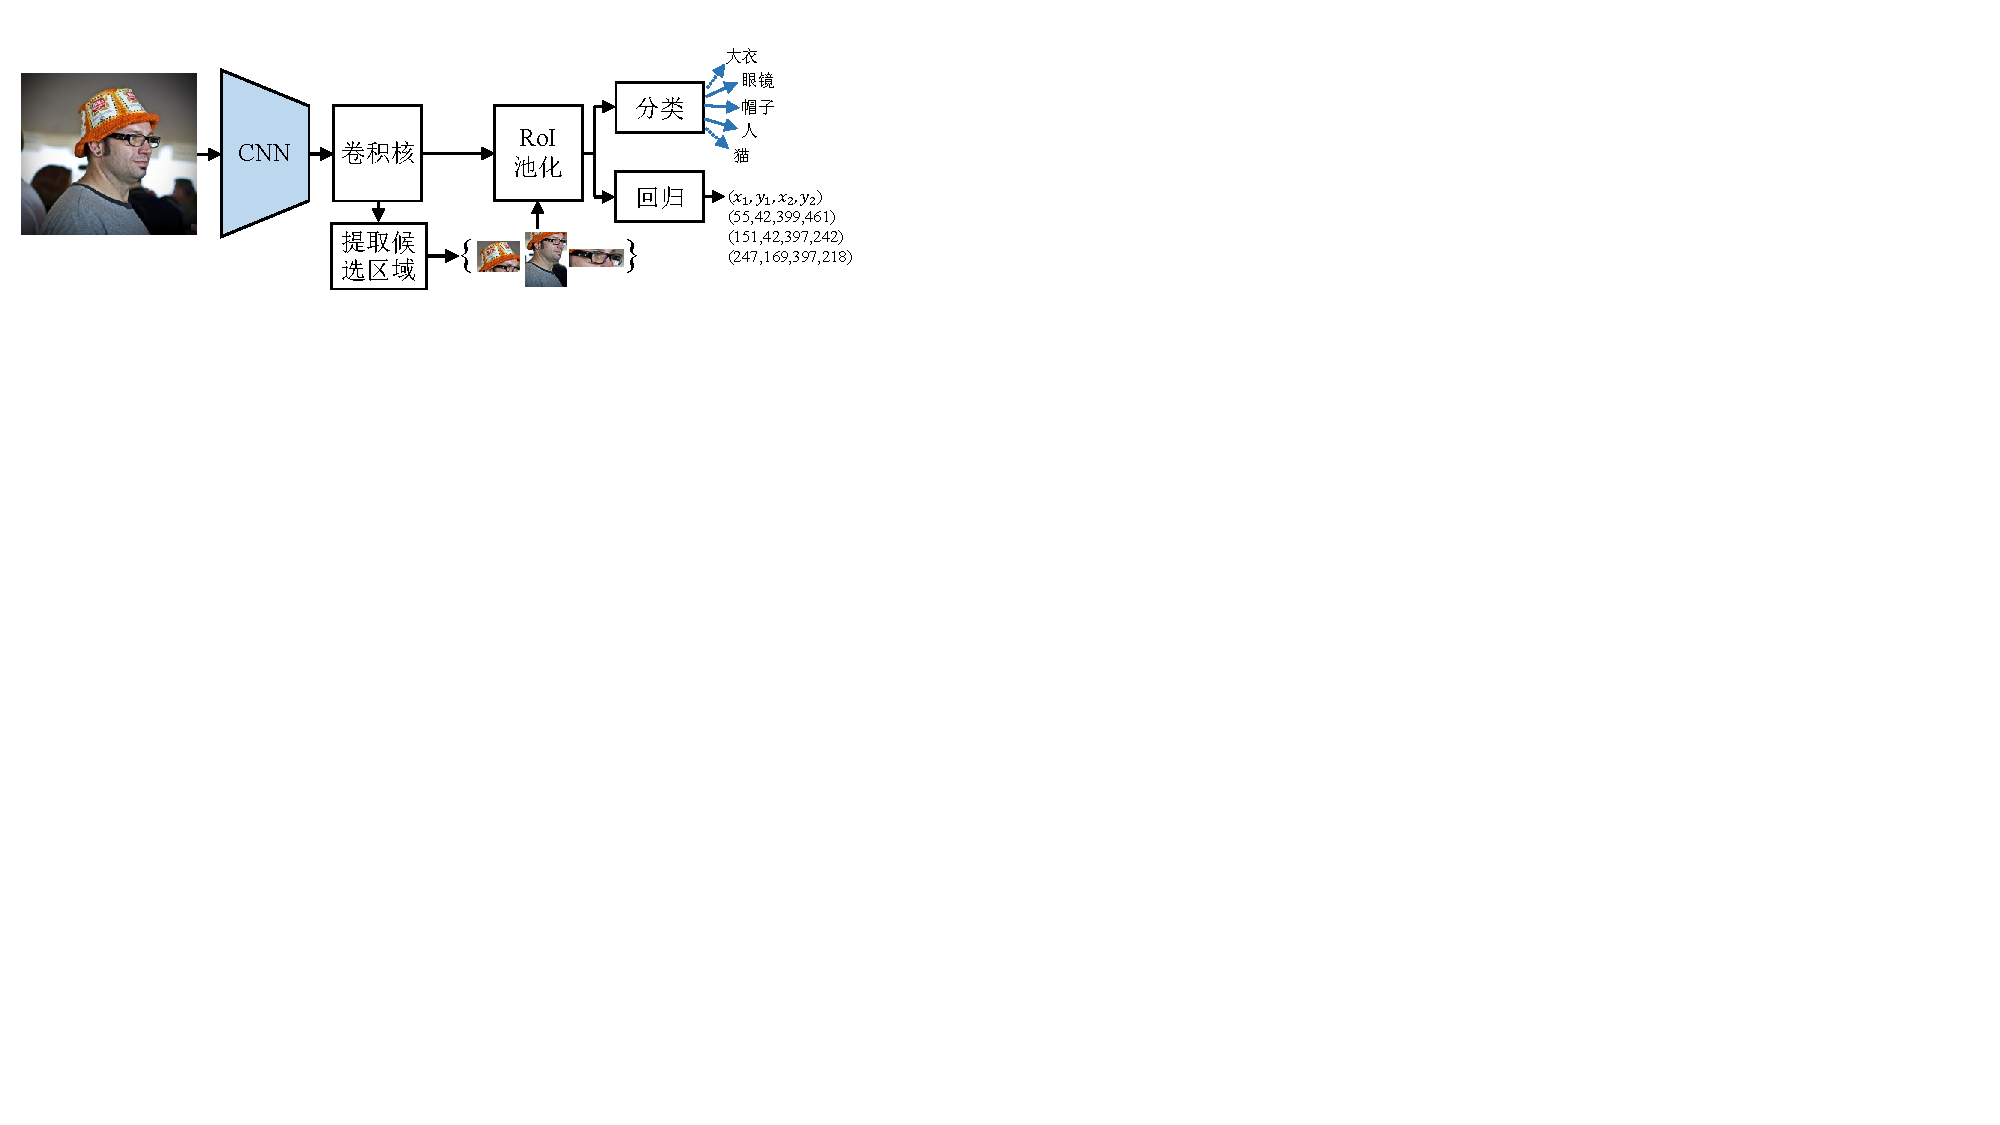
\includegraphics[scale=1.0]{Img/fig_2_rcnn.pdf}
      \caption{两阶段目标检测算法简图}
      \label{fig:2_rcnn}}
    \end{subfigure}%
    \\% line break
    \begin{subfigure}[b]{\textwidth}
      \centering
      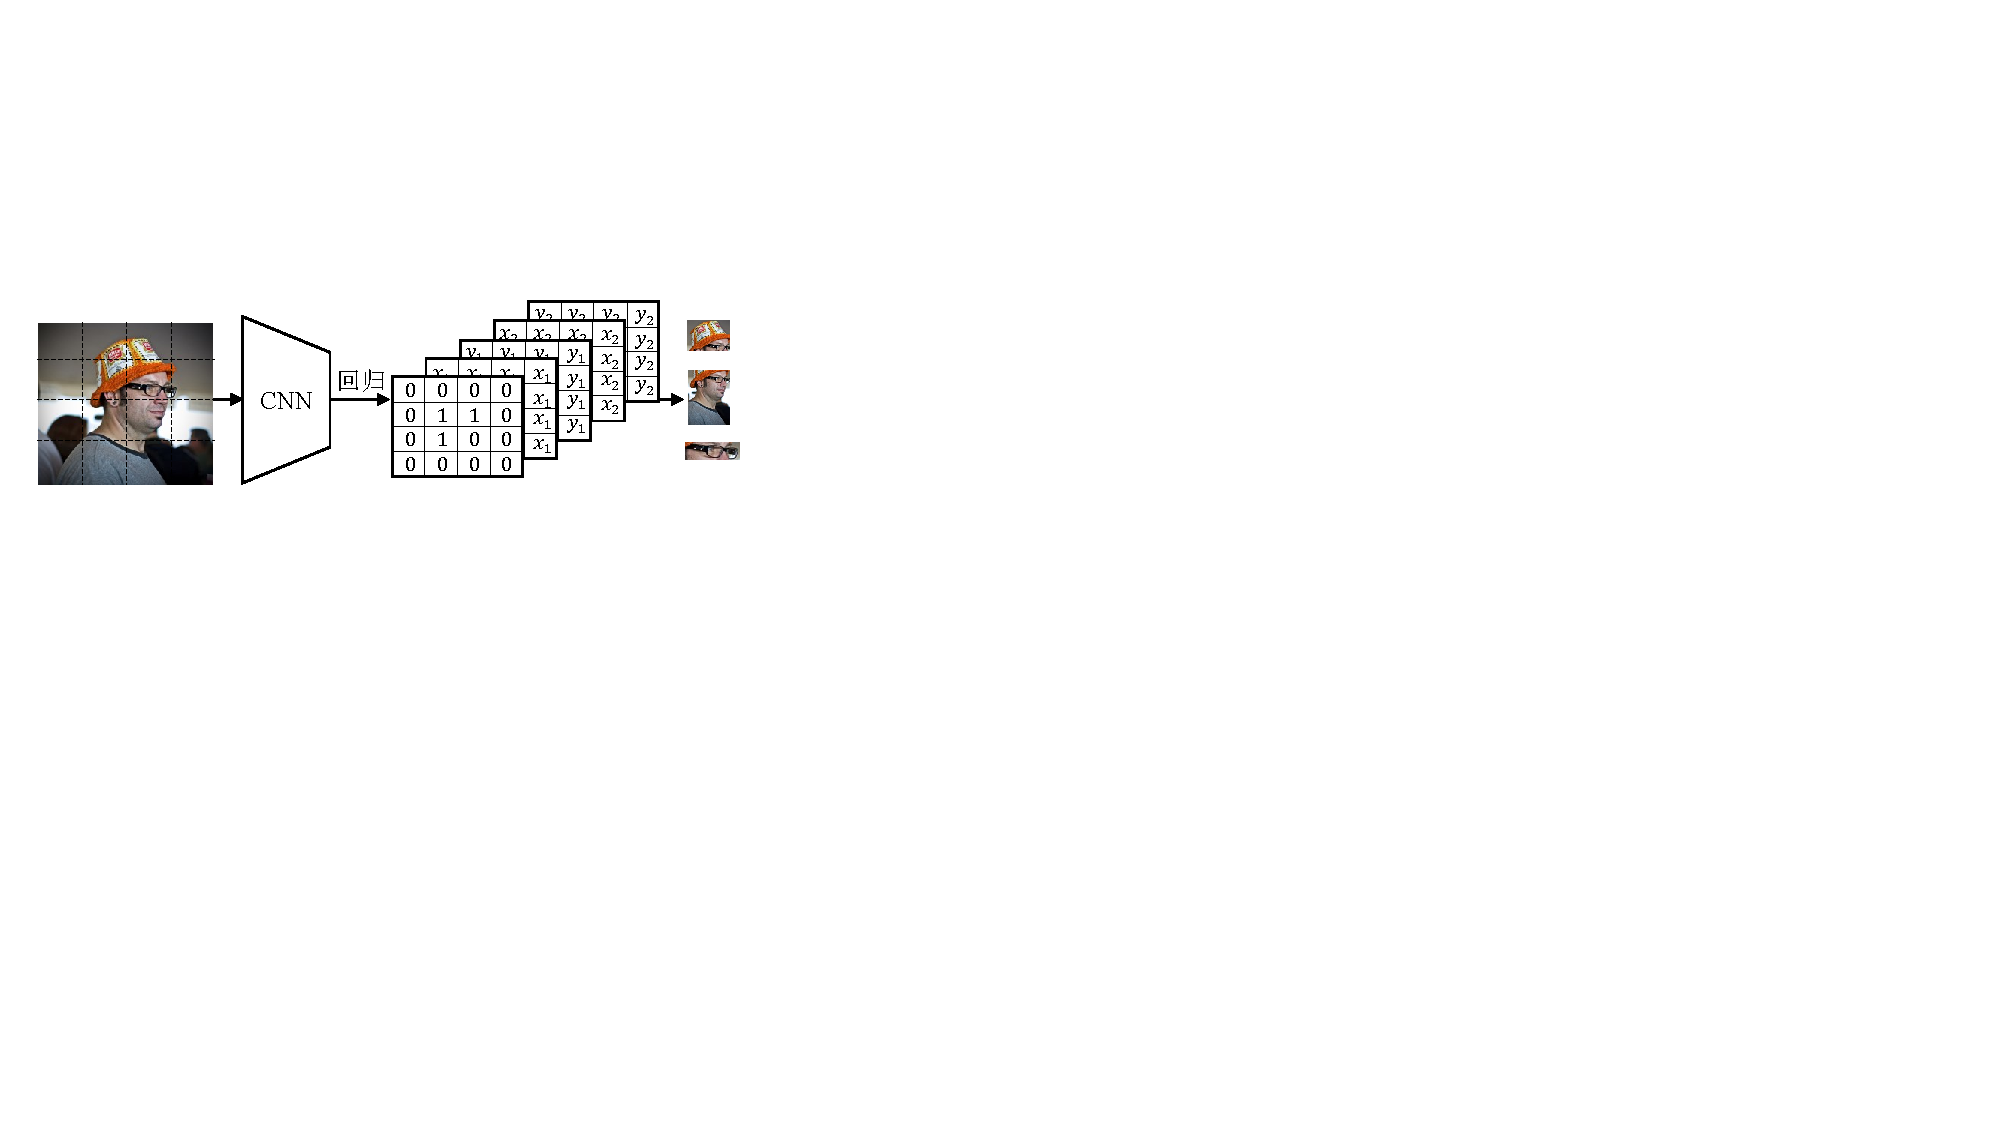
\includegraphics[scale=1.0]{Img/fig_2_yolo.pdf}
      \caption{一阶段目标检测算法简图}
      \label{fig:2_yolo}
    \end{subfigure}
    \\% line break
    \begin{subfigure}[b]{\textwidth}
      \centering
      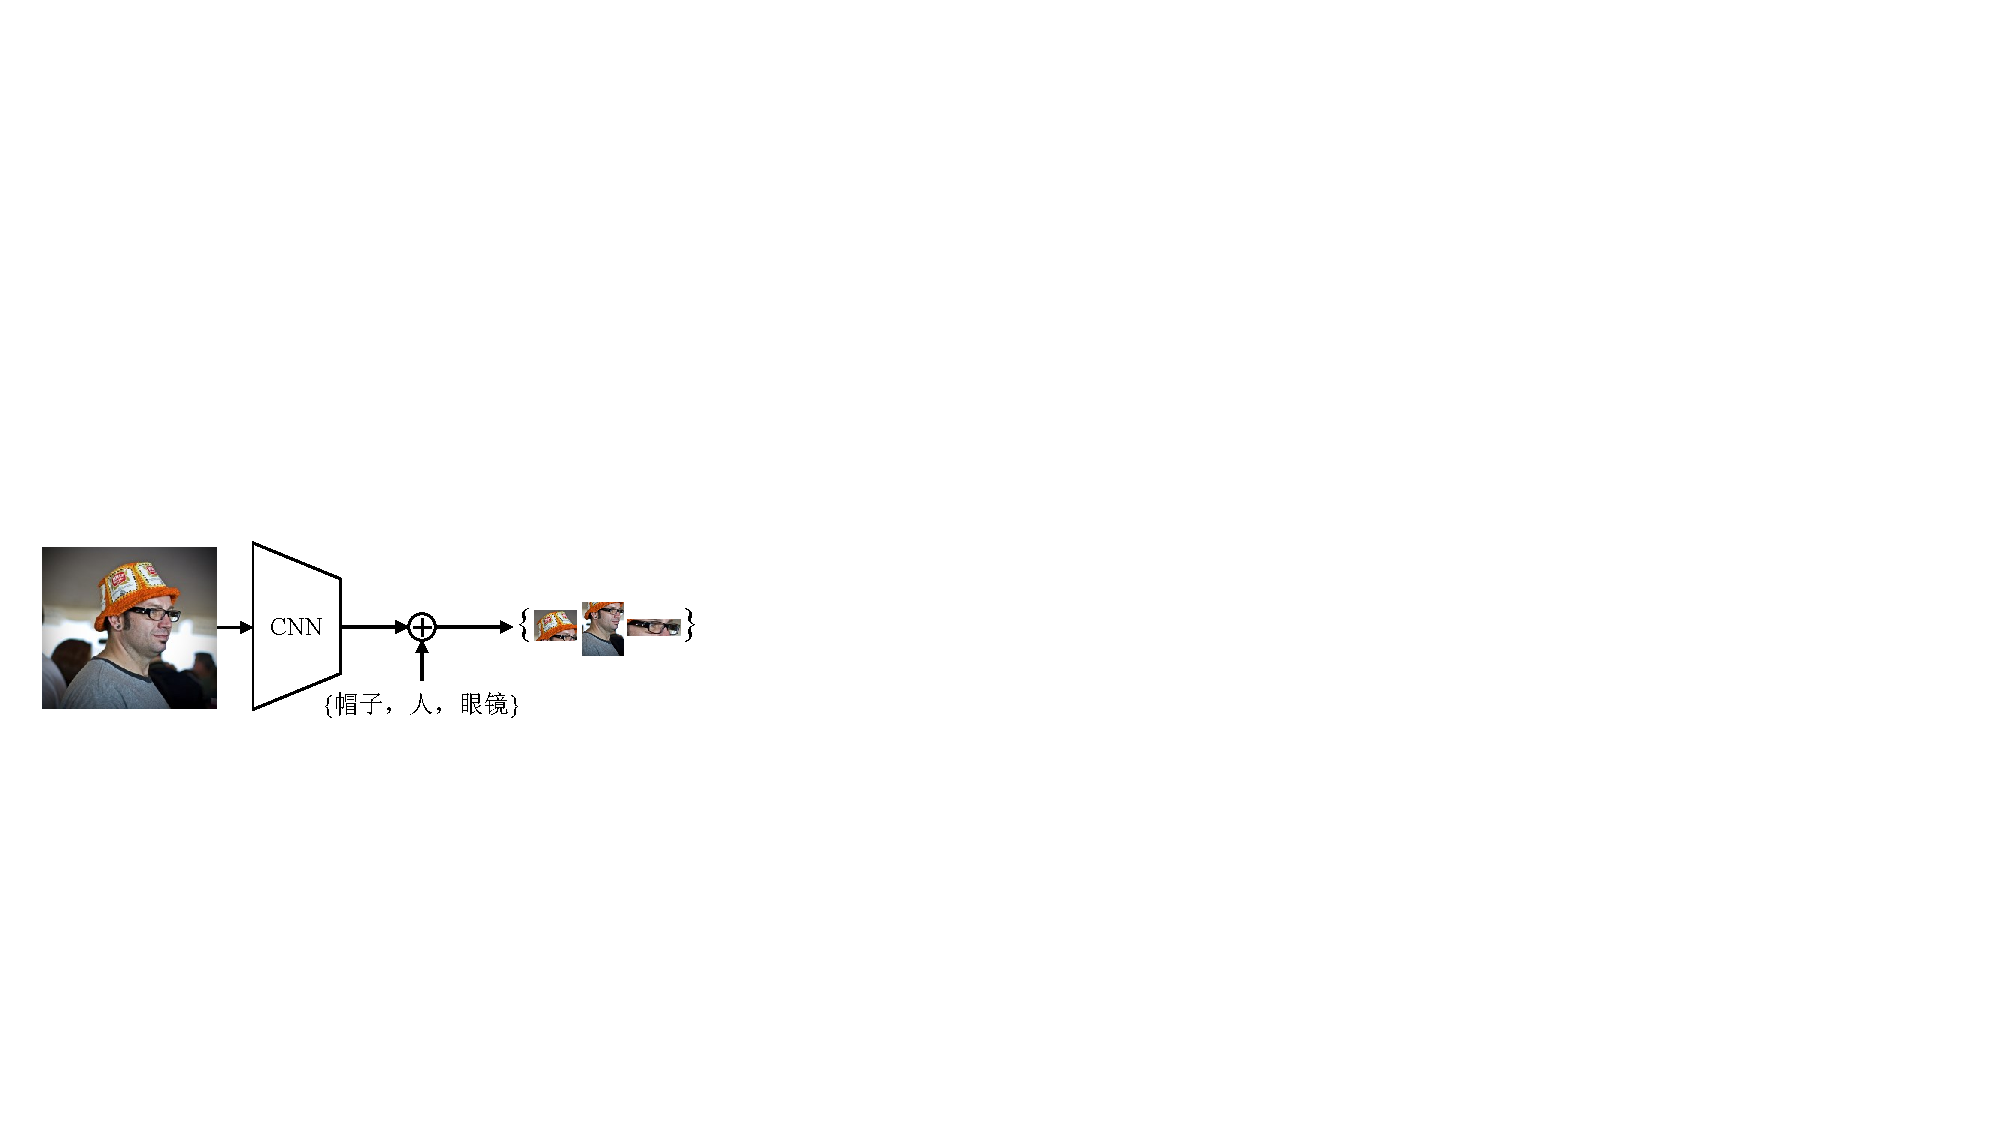
\includegraphics[scale=1.0]{Img/fig_2_visual_grounding.pdf}
      \caption{语义目标提取法简图}
      \label{fig:2_visual_grounding}
    \end{subfigure}%
    \bicaption{目标检测算法示意图}{Schematic diagram of object detection algorithm}
    \label{fig:2_object_detection}
\end{figure}
%方法背景介绍
目标检测是计算机视觉领域中一个应用范围非常广的任务,其目的是在图像或视频中自动地定位并识别出特定的视觉目标,从而满足对视觉目标的筛选、分类、追踪等需求。早期的目标检测算法需要手工设计特征和分类器来实现物体检测,并且运行速度较慢。随着深度学习的发展,目标检测算法开始采用卷积神经网络作为基础模型实现对视觉目标的检测,并取得了很好的性能与速度。对于融合图片信息的神经机器翻译任务,目标检测同样是非常重要的应用手段之一。与卷积神经网络能够提供图片的全局特征和栅格特征相比,目标检测的结果能够直接将图片中最有价值的前景信息提供给翻译模型。并且,每个视觉目标都能够提供排除与视觉目标不相关的更集中的视觉信息。

根据各算法特点以及工作方式,可以将目前常用的目标检测算法可以分为三类:两阶段法、一阶段法、语义目标提取法(visual grounding)。其中两阶段法和一阶段法提取给定图片中的所有类别可知的目标,并将提取出的目标分到相应的类别。语义目标提取法是根据语义信息提取相应的视觉目标,因此可以与前两者区分开。

{\sffamily (1)两阶段法}

两阶段法的代表方法有R-CNN(region-based convolutional neural networks)\pcite{girshick2014rich}、Fast R-CNN\pcite{girshick2015fast}以及Faster R-CNN\pcite{ren2015faster},如图\ref{fig:2_rcnn}。这类算法在目标检测过程中通常分为提取候选区域(region proposal)和特征提取与分类回归两个阶段。
从图片中提取视觉目标的最简单方式就是采用滑动窗口方法遍历图片中所有的矩形区域,然后利用分类器将有效的矩形区域分类到与其对应的类别。很显然,这种枚举的做法会消耗大量的检测时间。因此常见的两阶段法都会采用精心设计的算法提取出图片中的部分候选区域。例如,在R-CNN中采取了选择性搜索(selective search)算法在原始图片中提取出1000至2000个候选区域,也称感兴趣区域(region of interest,RoI),这种做法的弊端就是需要对这些候选区域都进行一次CNN的编码,同样耗费很多时间。而Fast RC-NN为了节省这部分时间先将图片经过CNN表征后再利用其所设计的RoI池化方法将栅格特征中与RoI相对应的区域提取出来。为了跟进一步地提高效率,Faster R-CNN方法采用了区域提取网络(region proposal network,RPN)代替耗时的选择性搜索算法。
通过第一阶段的提取就可以得到每个RoI的特征表示了,采用深度学习算法之前都是通过人工设计的特征来表征图片,而目前都是通过CNN来更方便的表征图像信息。将RoI的特征表示经过分类器就可以判断当前RoI是否属于某个已知的类别从而完成对提取到的视觉目标的分类。同时还要经过回归算法来获得目标的更精确的方框定位(bounding box)。

{\sffamily (2)一阶段法}

一阶段法的代表方法为YOLO(you only look once)\pcite{redmon2016you,redmon2017yolo9000,redmon2018yolov3,bochkovskiy2020yolov4,ge2021yolox}系列算法,其特点是采用单个神经网络同时完成对图像中视觉目标的提取和分类,而不需要预先生成候选区域。因此,一阶段法具有更快的目标检测速度。图\ref{fig:2_yolo}展示了YOLO算法的简化示意图,其基本工作原理是直接采用回归的方式替代预提取和分类的组合方式,利用CNN的对图像的表征回归图片中的方框坐标$(c,x_1,y_1,x_2,y_2)$,从而达到仅需要进行一次CNN的前向计算就能够得到检测结果的目的,其中$c$代表预测的置信度(confidence),$(x_1,y_1)$与$(x_2,y_2)$分别代表方框的左上角和右下角在图片中的位置坐标。为了能够一次提取图片中的多个视觉目标,则将输入图片划分为多个区域,每个区域负责一个视觉目标的提取。当视觉目标的中心落在某个区域时,该区域负责对该视觉目标的提取,例如图\ref{fig:2_yolo}中,图片被虚线分割的每个矩形区域与矩阵中每个位置一一对应,矩阵中“1”的位置分别对应了图片中“人”、“帽子”和“眼镜”的中心所在的矩形区域。

{\sffamily (3)语义目标提取法}

在图片中提取与文本语义相关区域的方法是语义目标提取法,方法示意图如图\ref{fig:2_visual_grounding}所示。这类方法的输入是一张完整的图片和需要提取内容的文本。例如提取图片中的“人”时,其模型输入为图片和文本“人”、“男人”或者“一个戴眼镜的男人”。提取视觉目标的过程需要对图片和文本先编码,然后将利用跨模态信息融合的方式识别出图片中与文本语义最相近的区域。最初的语义目标提取可以认为是目标检测任务的下游任务,所用的方法是先采用常用的目标检测方法将图中的视觉目标提取出来并分类。然后根据视觉目标类别与输入文本相似度通过匹配的方式完成语义目标的提取。这种传统的语义目标提取方法因为需要两种方法相结合才能完成任务,因此也称为两阶段法。而图\ref{fig:2_visual_grounding}中所展示的方法不需要先提取再匹配的过程,所有提取步骤在一个统一的模型中完成,因此称为一阶段法。采用语义目标提取法获得视觉目标的方式能够将文本的内容与图片中的视觉目标对应起来,对于跨模态信息融合有很大的帮助。本文在后面的章节\ref{sec:3_entity_extraction}小节所介绍的工作就采用了一种一阶段的语义目标提取法,来获取句子中的短语与图片中的视觉目标的对应关系。
%方法介绍

%在ImgNMT中的应用

%对于跨模态信息融合,目标检测依旧是非常重要的应用手段之一。与卷积神经网络相比,目标检测的结果能够直接将图片中那些信息量最大的目标直接提供给翻译模型,而提取出的视觉目标所包含的信息也更集中。目标检测的结果可以分为两种,一种是检测结果与文本不建立关系,此时目标检测方法输出的多个视觉目标结果可以视为视觉目标序列输入到以序列建模擅长的自然语言处理任务的模型中。另一种是通过文本语义进行视觉目标检测,这种方式能够对齐文本与视觉目标,更方便在翻译中使用。
% 目标检测要给出区域,和分类
% 最初的设定,扫描图片中的所有框
% R-CNN:two-stage,ROI->feature extraction for ROI->SVM->位置精修
%      R-CNN-> Fast R-CNN -> Faster R-CNN
% Yolo v0-5: one-stage (you only look once)(regression)
%      v0: 遍历所有“框” -》 输出(c,x,y,w,h) 其中c为confidence,label为(1,x*,y*,w*,h*)
%      v1:检测多个目标,将img划分为多个区域,(c,x,y,w,h,one-hot)*N
% visual grounding

%\subsection{视觉Transformer}
%这里和前面呼应以下,前面是CV推动着NLP的发展,这里则反过来,NLP推动CV

%预示着大模型的融合

%与CNN相同同样可以做backbone,做目标检测以及图片分类

% 结尾说以下那几篇文章说过使用哪种CNN-backbone带来的差别并不大